\documentclass{report}
\usepackage{tocloft}
\usepackage{geometry}
\usepackage{graphicx}
\usepackage{caption}
\usepackage[T1]{fontenc}
\usepackage[utf8]{inputenc}
\usepackage[polish]{babel}
\usepackage{float}
\usepackage{listings}
\usepackage{xcolor}

\geometry{
    a4paper,
    left=2.5cm,
    right=2.5cm,
    top=2.5cm,
    bottom=2.5cm,
}

\lstset{
    language=Matlab,
    basicstyle=\footnotesize\ttfamily,
    keywordstyle=\color{blue},
    commentstyle=\color{green},
    stringstyle=\color{red},
    numbers=left,
    numberstyle=\tiny\color{gray},
    stepnumber=1,
    numbersep=5pt,
    backgroundcolor=\color{lightgray},
    frame=single,
    tabsize=2,
    captionpos=b,
    breaklines=true
}


\setcounter{tocdepth}{3}
\setlength{\cftbeforechapskip}{15pt} 
\setlength{\cftbeforesecskip}{8pt} 
\setlength{\cftbeforesubsecskip}{5pt} 
\setlength{\cftbeforesubsubsecskip}{5pt}

\renewcommand\thesection{\arabic{section}.}
\renewcommand\thesubsection{\thesection\arabic{subsection}.}
\renewcommand\thesubsubsection{\thesubsection\arabic{subsubsection}.}
\setcounter{secnumdepth}{3}


\begin{document}


\begin{titlepage}
    \centering
    \vspace*{1cm}
    \begin{figure}
        \centering 
        \includegraphics[width=0.5\textwidth]{"logo.png"}
    \end{figure}
    \Huge
    Zajęcia Projektowe
    \par
    \textbf{Oprogramowanie Systemów Pomiarowych}
    
    \vspace*{1cm}

    \vspace{0.5cm}
    \LARGE \textit{Aplikacja autoryzacji dostępu oparta 
    na biometrycznej weryfikacji tożsamości}
    
    \vspace{1.5cm}
    
    \textbf{Autorzy:} 
    \par
    Jakub Pająk 
    \par
    Łukasz Grabarski
    \par 
    Krzysztof Grądek
    \par 
    Piotr Legień
    \vspace*{1.5cm}
    \par AiR Grupa 5TI
    
    \vfill
    
    \Large 16.05.2024
    
\end{titlepage}


\newpage

\tableofcontents

\newpage


\section{\LARGE Wprowadzenie}
\subsection{\Large Cel projektu}
Celem projektu była implementacja aplikacji mającej główną część logiki osadzoną w środowisku progtamistycznym 
LabView oraz napisanie skryptu w języku Python realizującego rozpoznawanie twarzy w celu autoryzacji dostępu. 


\subsection{\Large Założenia wstępne}
Wstępne odgórne założenia implikowały wykorzystanie środowiska programistycznego LabView z szczególnym warunkiem jakim było wykorzystanie 
maszyny stanów JKI - jednego z znaczących framework-ów LabView. 

Rdzeń aplikacji winien był być osadzony w wcześniej wymienionej maszynie stanów. 
Kolejnym wymaganiem było napisanie odpowiedniej funkcji w języku Python porównującej pobrane zdjęcie podczas próby logowania z zdjęciami znanych użytkowników.
Ponadto należało zaimplementować prostą bazę danych do zarządzania znanymi użytkownikami oraz ich danymi. 

\subsection{\Large Harmonogram realizacji projektu}
\subsubsection{\large Okres 1}
Zaprojektowanie podstawowego interfejsu użytkownika w środowisku LabVIEW. Dodanie stosownych pól 
oraz przycisków umożliwiających późniejsze logowanie oraz nawigację po aplikacji.

\subsubsection{\large Okres 2}
Zapoznanie się z sposobem połączenia oraz wywołania skryptu napisanego w języku Python z poziomu środowiska LabView.
Implementacja podstawowej wersji skryptu zdolnego do poprawnego porówniania dwóch obrazów zawierających twach potencjalnego użytkownika.
Próba wywołania skryptu w aplikacji LabView.

\subsubsection{\large Okres 3}
Dostosowanie skryptu do odpowiednich folderów oraz zmiana implementacji tak, aby kod sprawdzał czy użytkownik próbujący zalogować się do aplikacji widnieje wśród użytkowników 
znanych, czyt. uprzednio dodanych do folderu.
Zapoznanie się z sposobem połączenia apliakcji LabView z relacyjną bazą danych SQL Server.

\subsubsection{\large Okres 4}
Wdrożenie połączenia z bazą danych oraz weryfikacja poprawności połączenia przy wykorzystaniu podstawowych operacji takich jak SELECT lub INSERT.
Testy aplikacji.

\section{\LARGE Dokumentacja aplikacji}

\subsection{\Large Zagadnienia ogólne oraz środowiska programistyczne}
Aplikacja została zrealizowana w zaawansowanym środowisku programistycznym produkowanym przez firmę National Instruments, znanym jako LabView. Jest to blokowy język programowania, który umożliwia stosunkowo szybkie tworzenie szerokiej gamy aplikacji. Obszerna paleta dostępnych rozszerzeń oraz dodatkowych pakietów znacząco zwiększa efektywność pracy w języku LabView. Wiele złożonych zagadnień można rozwiązać za pomocą kilku elementów z odpowiednich bibliotek. Jednakże, ze względu na nietypowy sposób tworzenia programów w LabView, okres adaptacji do tego nowego środowiska może być nieco dłuższy.

Drugim środowiskiem programistycznym, które zostało wykorzystane, jest Python w wersji 3.10. Szczegółowe uzasadnienie wyboru tej konkretnej dystrybucji języka zostanie przedstawione w dalszych częściach dokumentacji. Podobnie jak LabView, język Python umożliwia dostęp do szerokiej gamy gotowych rozwiązań, które umożliwiają rozwiązywanie złożonych problemów. W związku z tym, w projekcie zastosowano bibliotekę OpenCV wraz z nowoczesnym pakietem face-recognition. Wykorzystanie tych pakietów sprawiło, że implementacja logiki rozpoznawania twarzy stała się zadaniem prostym i efektywnym.

Trzecim środowiskiem programistycznym, jakie zostało użyte, jest SQL Server w połączeniu z systemem SQL Management Studio (SSMS). Ostatni element aplikacji, polegający na dodaniu bazy danych do środowiska LabView, został zrealizowany przy użyciu tych narzędzi. Proces ten nie był tak prosty, jak mogłoby się wydawać na pierwszy rzut oka, dlatego zostanie dokładnie omówiony w odpowiedniej sekcji dokumentacji.


\subsection{\Large Omówienie szkieletu aplikacji - Framework LabView JKI}

Framework LabView JKI jest zaawansowanym zestawem narzędzi oraz wzorców projektowych stworzonych z myślą o usprawnieniu procesu tworzenia aplikacji w środowisku LabView. Jest on szczególnie ceniony za swoje podejście modularne, które umożliwia tworzenie skalowalnych i łatwych do utrzymania aplikacji.

\subsubsection*{Struktura Frameworka}

Framework LabView JKI charakteryzuje się jasno zdefiniowaną strukturą, która ułatwia organizację kodu. Składa się z modułów, które są niezależnymi jednostkami funkcjonalnymi, co pozwala na efektywną separację zadań i logiki aplikacji. Moduły te mogą być łatwo integrowane i wymieniane, co zapewnia elastyczność w zarządzaniu projektem oraz wprowadzaniu zmian.

\subsubsection*{Zarządzanie zasobami i procesami}

Jednym z kluczowych aspektów frameworka JKI jest jego podejście do zarządzania zasobami i procesami. Wykorzystuje on wzorzec aktorów, gdzie każdy aktor reprezentuje autonomiczną jednostkę wykonawczą odpowiedzialną za konkretne zadania. Komunikacja pomiędzy aktorami odbywa się za pomocą wiadomości, co minimalizuje ryzyko konfliktów i zapewnia płynność operacji.

\subsubsection*{Efektywność i optymalizacja}

Framework JKI zawiera szereg narzędzi wspomagających optymalizację aplikacji. Dzięki wbudowanym mechanizmom monitorowania i debugowania, deweloperzy mogą szybko identyfikować i rozwiązywać problemy wydajnościowe. Ponadto, framework wspiera zarządzanie pamięcią oraz zasobami systemowymi, co jest kluczowe dla utrzymania wysokiej wydajności aplikacji nawet przy intensywnym obciążeniu.

\subsubsection*{Integracja z innymi technologiami}

Framework LabView JKI został zaprojektowany z myślą o łatwej integracji z innymi technologiami i systemami. Obsługuje różnorodne protokoły komunikacyjne oraz standardy wymiany danych, co umożliwia płynne połączenie z zewnętrznymi bazami danych, urządzeniami pomiarowymi oraz innymi aplikacjami. Dzięki temu, możliwe jest tworzenie kompleksowych rozwiązań, które są w stanie sprostać najbardziej wymagającym zadaniom.

\subsubsection*{Dokumentacja i wsparcie społeczności}

Framework JKI jest dobrze udokumentowany, co znacznie ułatwia naukę i wdrażanie jego elementów w projekcie. Obszerna dokumentacja zawiera szczegółowe opisy funkcji, przykłady kodu oraz najlepsze praktyki. Dodatkowo, aktywna społeczność użytkowników i deweloperów stanowi cenne źródło wsparcia oraz inspiracji, co jest szczególnie ważne w przypadku napotkania problemów lub wątpliwości.

\subsection{\Large Framework JKI - opis podstawowych stanów}
Sekcja ta ma na celu wprowadzenie użytkownika dla którego programowanie w LabVIEW, a w szczególności z wykorzystaniem framework-a JKI jest obce. 
Framework ten ma pewne elementy specyficzne dla siebie, a których rozumienie jest kluczowe w rozumieniu zasady działania aplikacji. 

Warto nadmienić, że bardzo pomocym narzędziem podczas korzystania z LabView jest Help - można użyć skrótu klawiszowego CTRL + H. 
Informacje zawarte w pomocy są często bardzo pomocne, jeśli nie wystarczają można przejść do linka "Detailed help", tam znajdują się bardzo szczegółowe informacje oraz niekiedy przykłady użycia.

\subsubsection{\large Ogólny wygląd schematu blokowego JKI}

\begin{figure} [H]
    \centering
    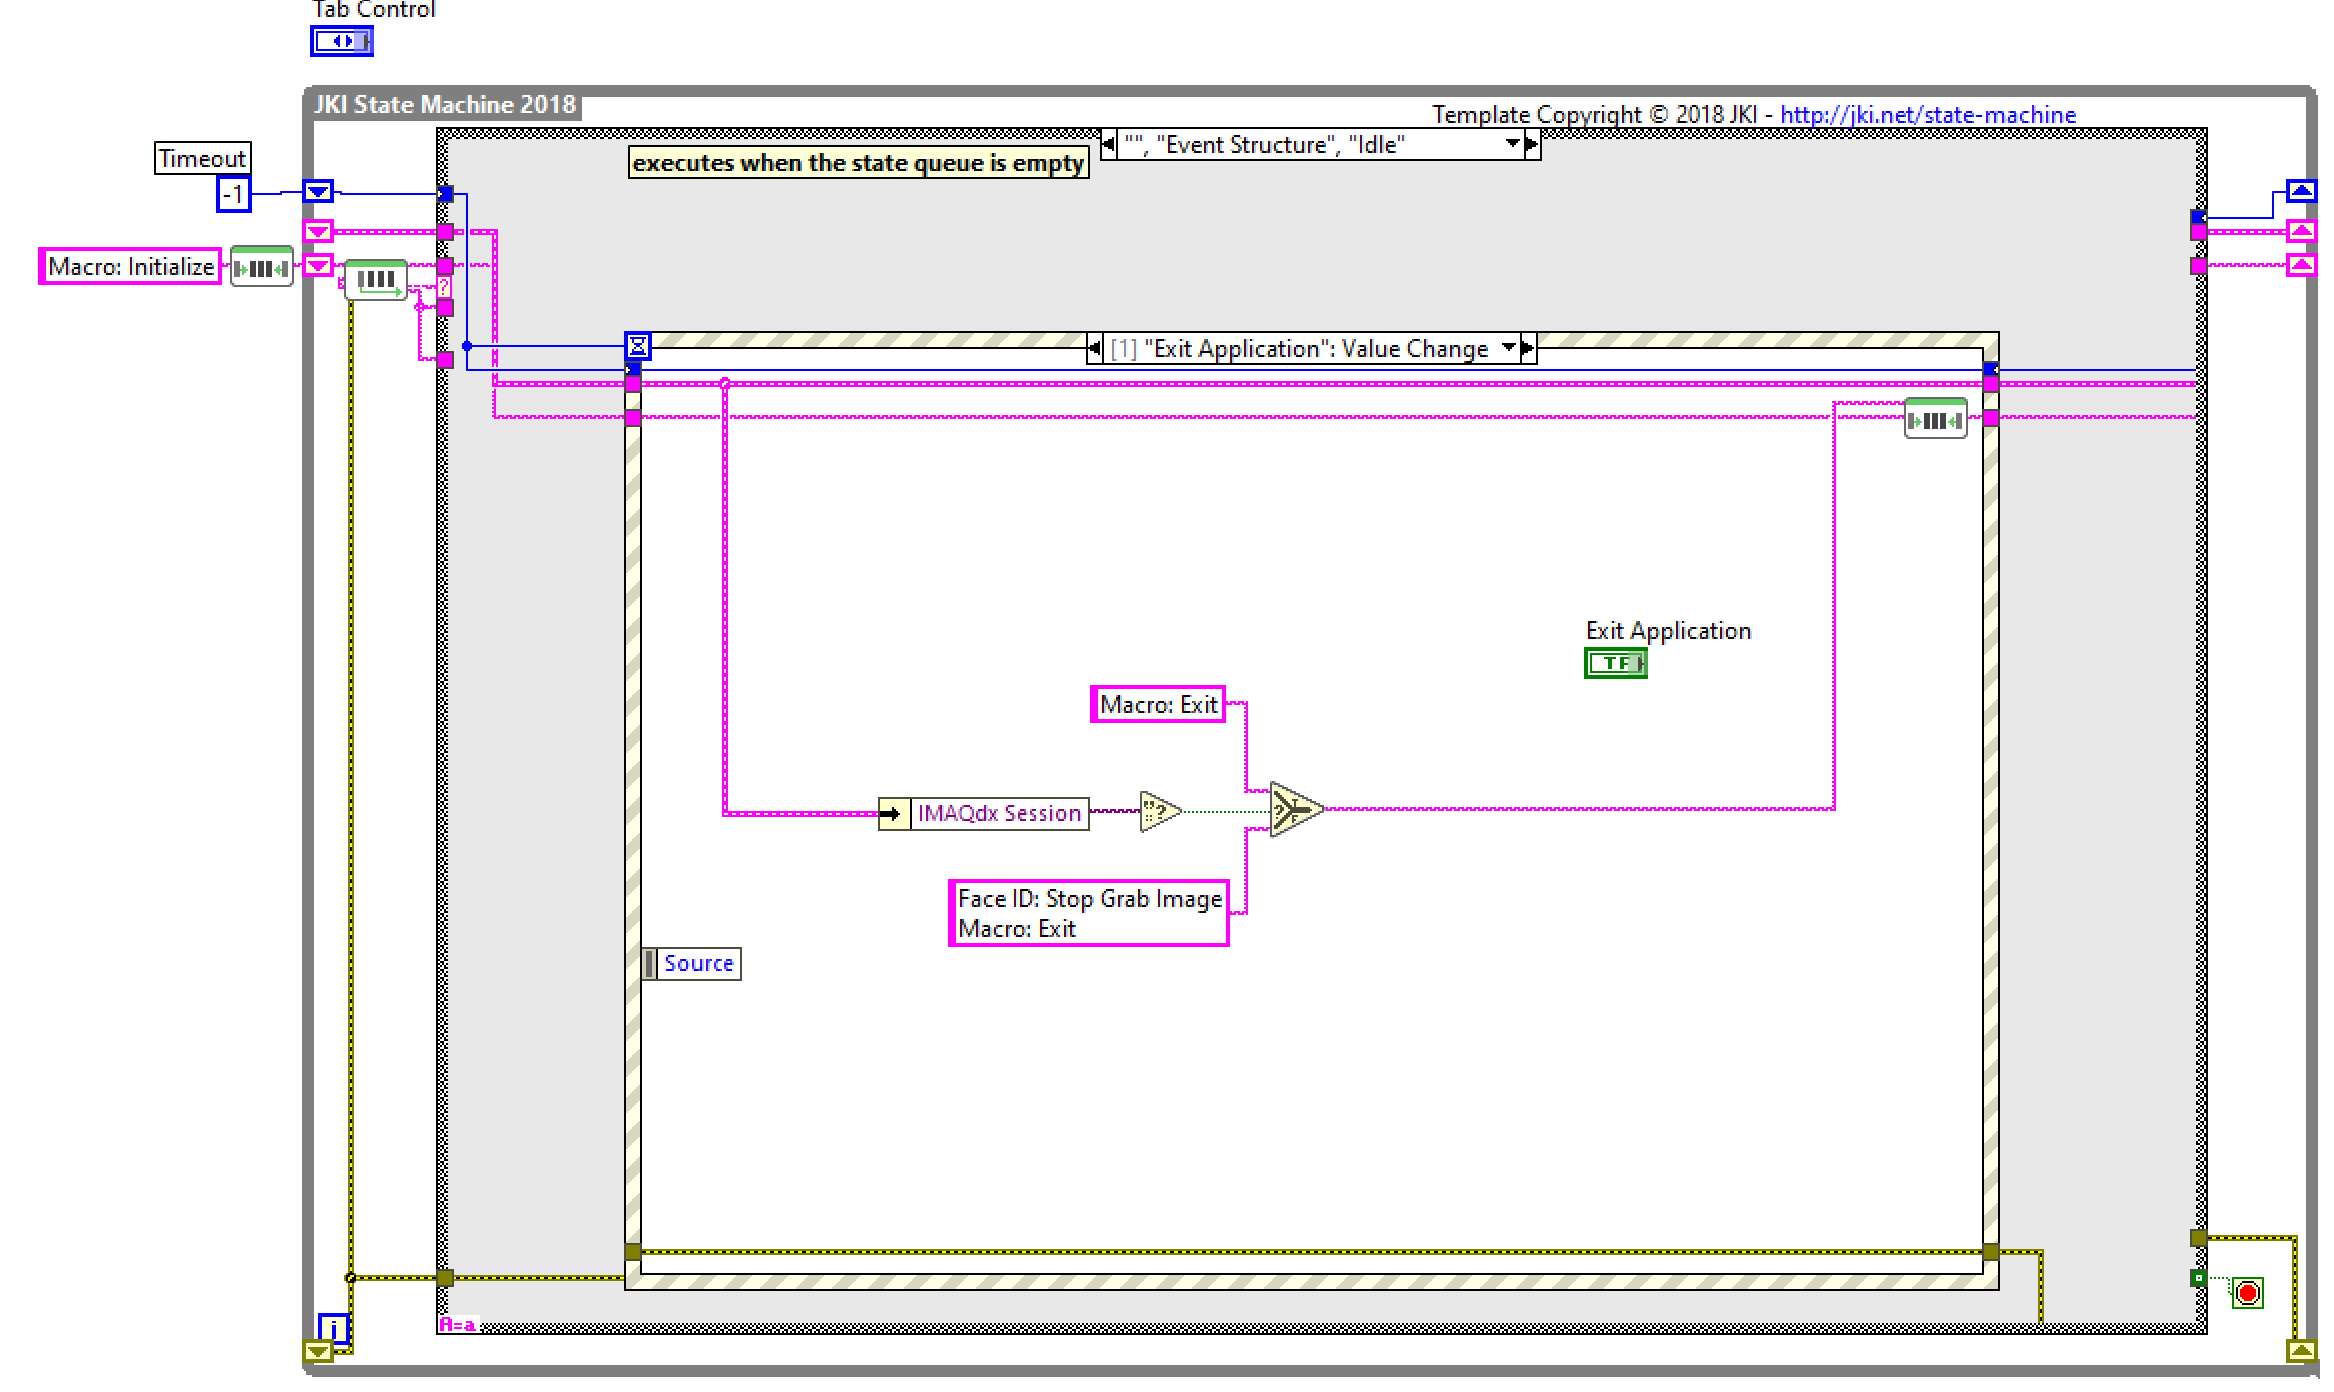
\includegraphics[width=1.0\textwidth]{"src/jki-main.png"}
    \caption{Zdjęcie przedstawiające podstawowy widok schemtu blokowego maszyny stanów JKI}
    \label{fig:foto1}
\end{figure}

Maszyna stanów JKI składa się z dwóch głównych elementów:
\begin{itemize}
    \item Pętli While,
    \item Struktury Case.
\end{itemize}

Pętla while odpowiada za nieskończone (naturalnie do momentu zdarzenia kończącego działania aplikacji) wykonywanie się aplikacji w pętli.
Podczas uruchomienia aplikacja rozpoczyna pracę w pętli oraz przechodzi przez kolejne stany (case) aplikacji.

Drugim elementem jest struktura Case, która odpowiada za naturę działania maszyny stanów - przechodzenie do odpowiednich stanów zdefiniowanych podczas uruchomienia oraz następnie zaciąganych z kolejki. 

\begin{figure} [H]
    \centering
    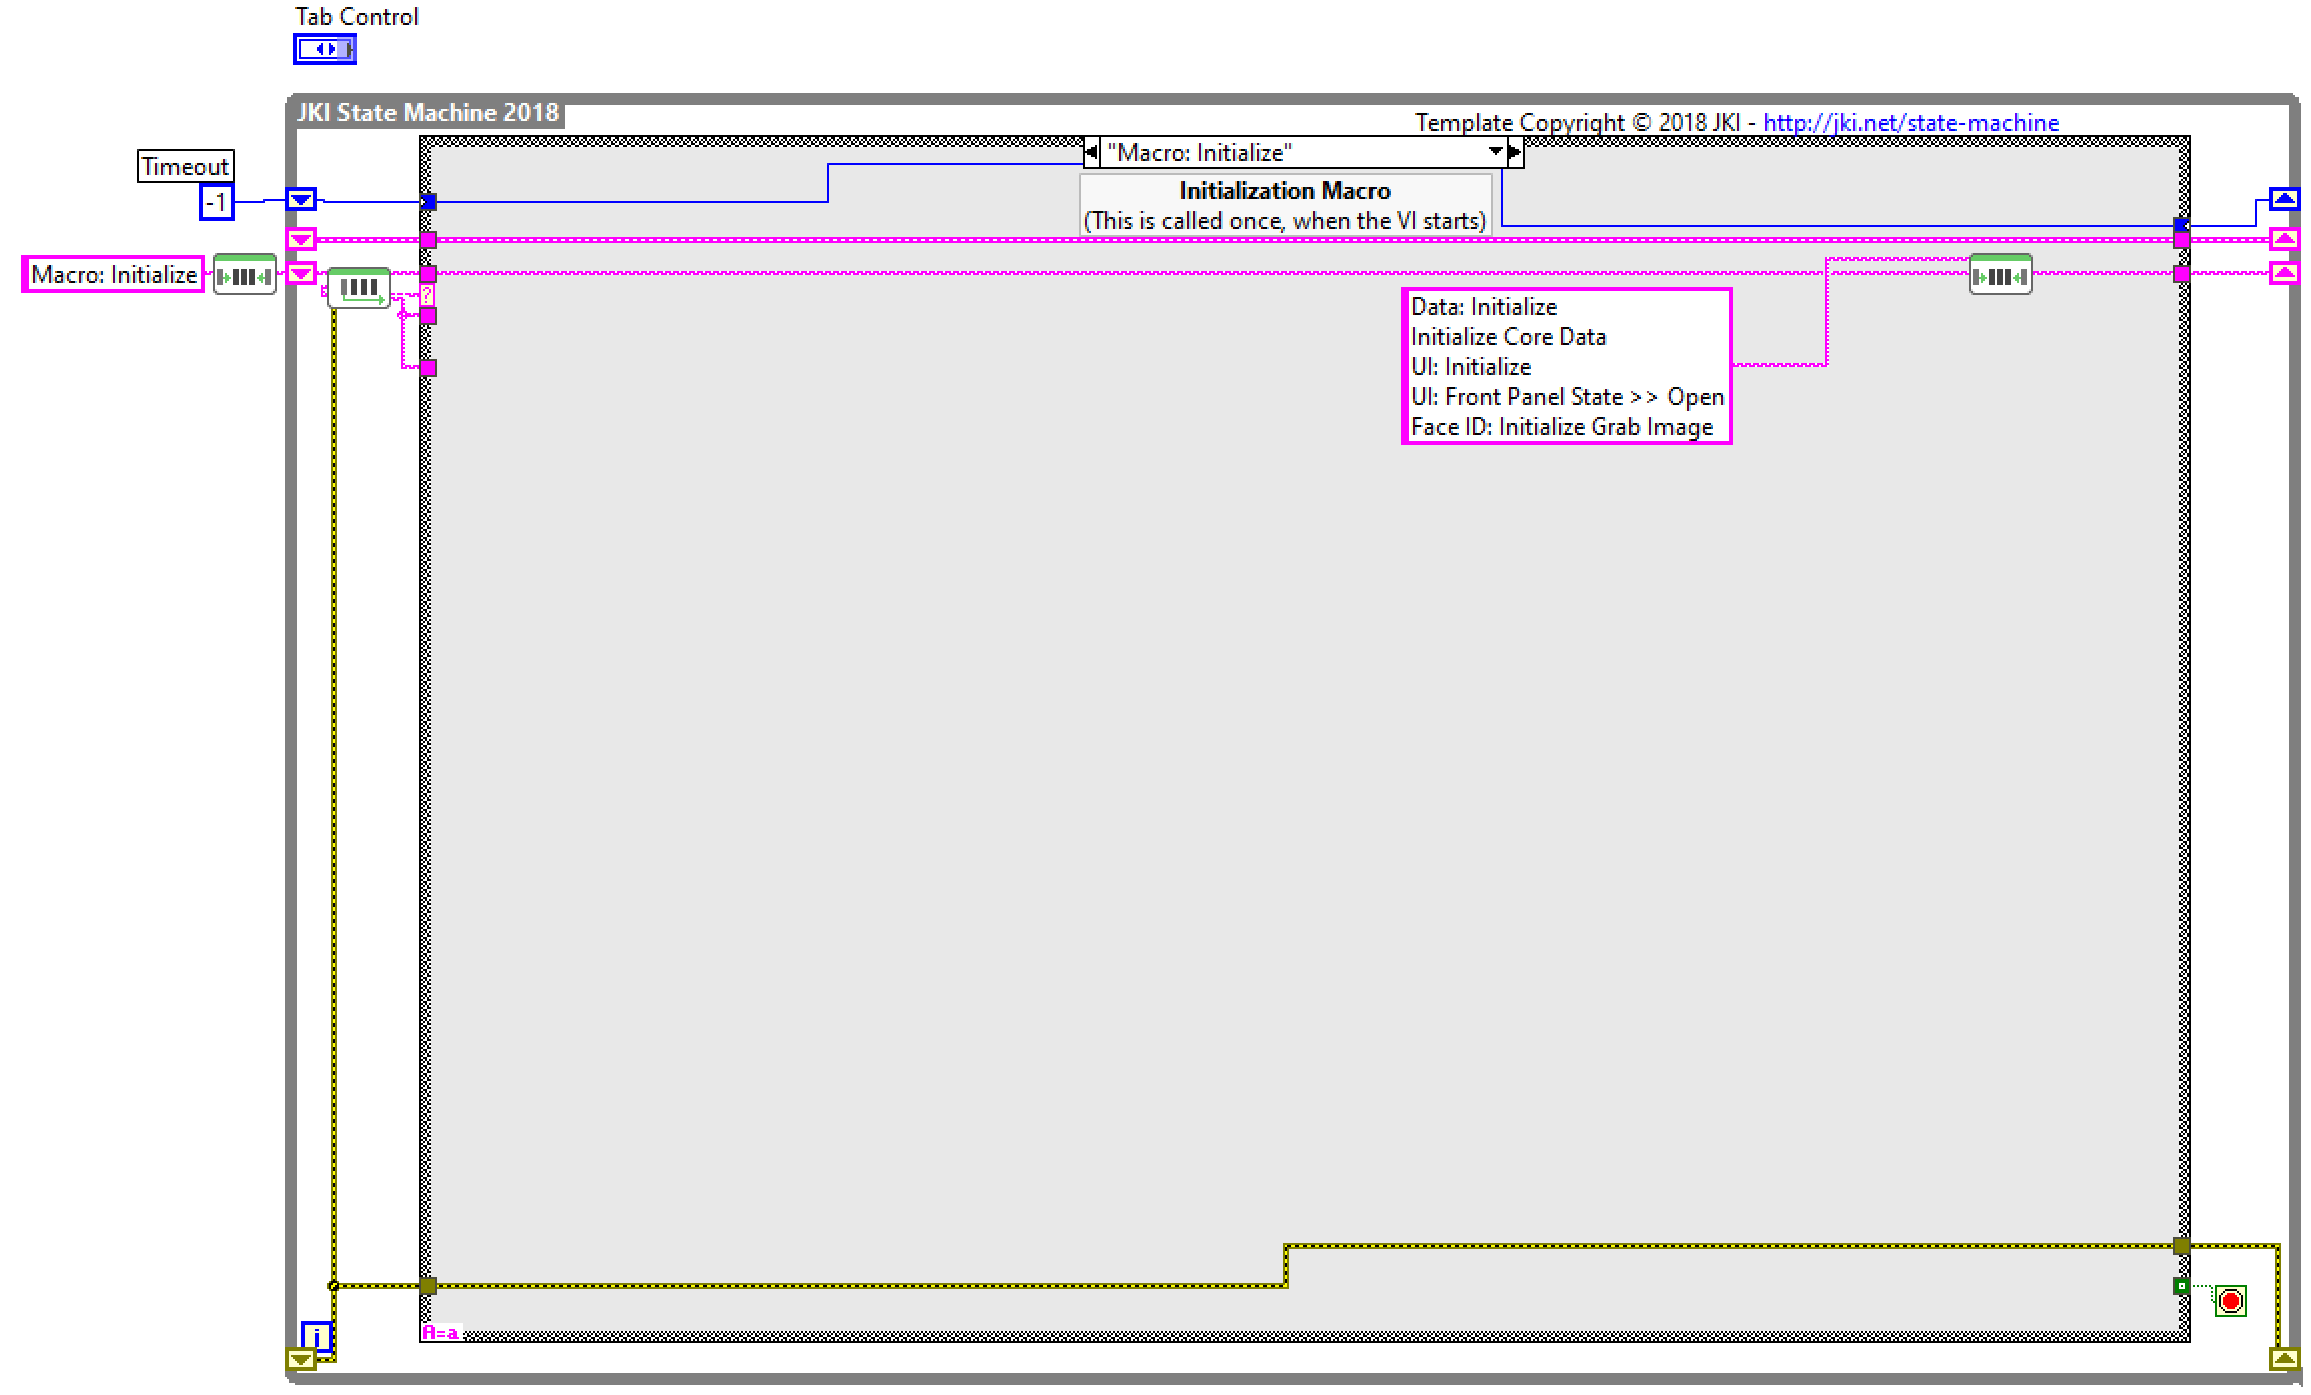
\includegraphics[width=1.0\textwidth]{"src/macro-init.png"}
    \caption{Zdjęcie przedstawiające stan "Macro: Initialize"}
    \label{fig:foto2}
\end{figure}

Stan "Macro: Initialize" jest wykonywany podczas startu aplikacji (jest to wyszczególnione pod rozwijaną listą ze stanami). Ważnym elementem jest pole statyczne typu String (oznaczone typowo kolorem różowym) 
zawierające pięć kolejnych stanów, które zostaną wysłane na kolejkę w celu odpowiedniego toku wykonywania. Najpierw wykona się stan Data: Initialize, następnie Initialize: Core Data etc. 
Na samym końcu zostanie wywołany stan Face ID: Initialize Grab Image. Jest to pierwszy stan, który nie jest zapewniony przez framework, a zatem kod napisany samodzielnie rozpoczyna się wraz z wywołaniem stanu piątego. 

\begin{figure} [H]
    \centering
    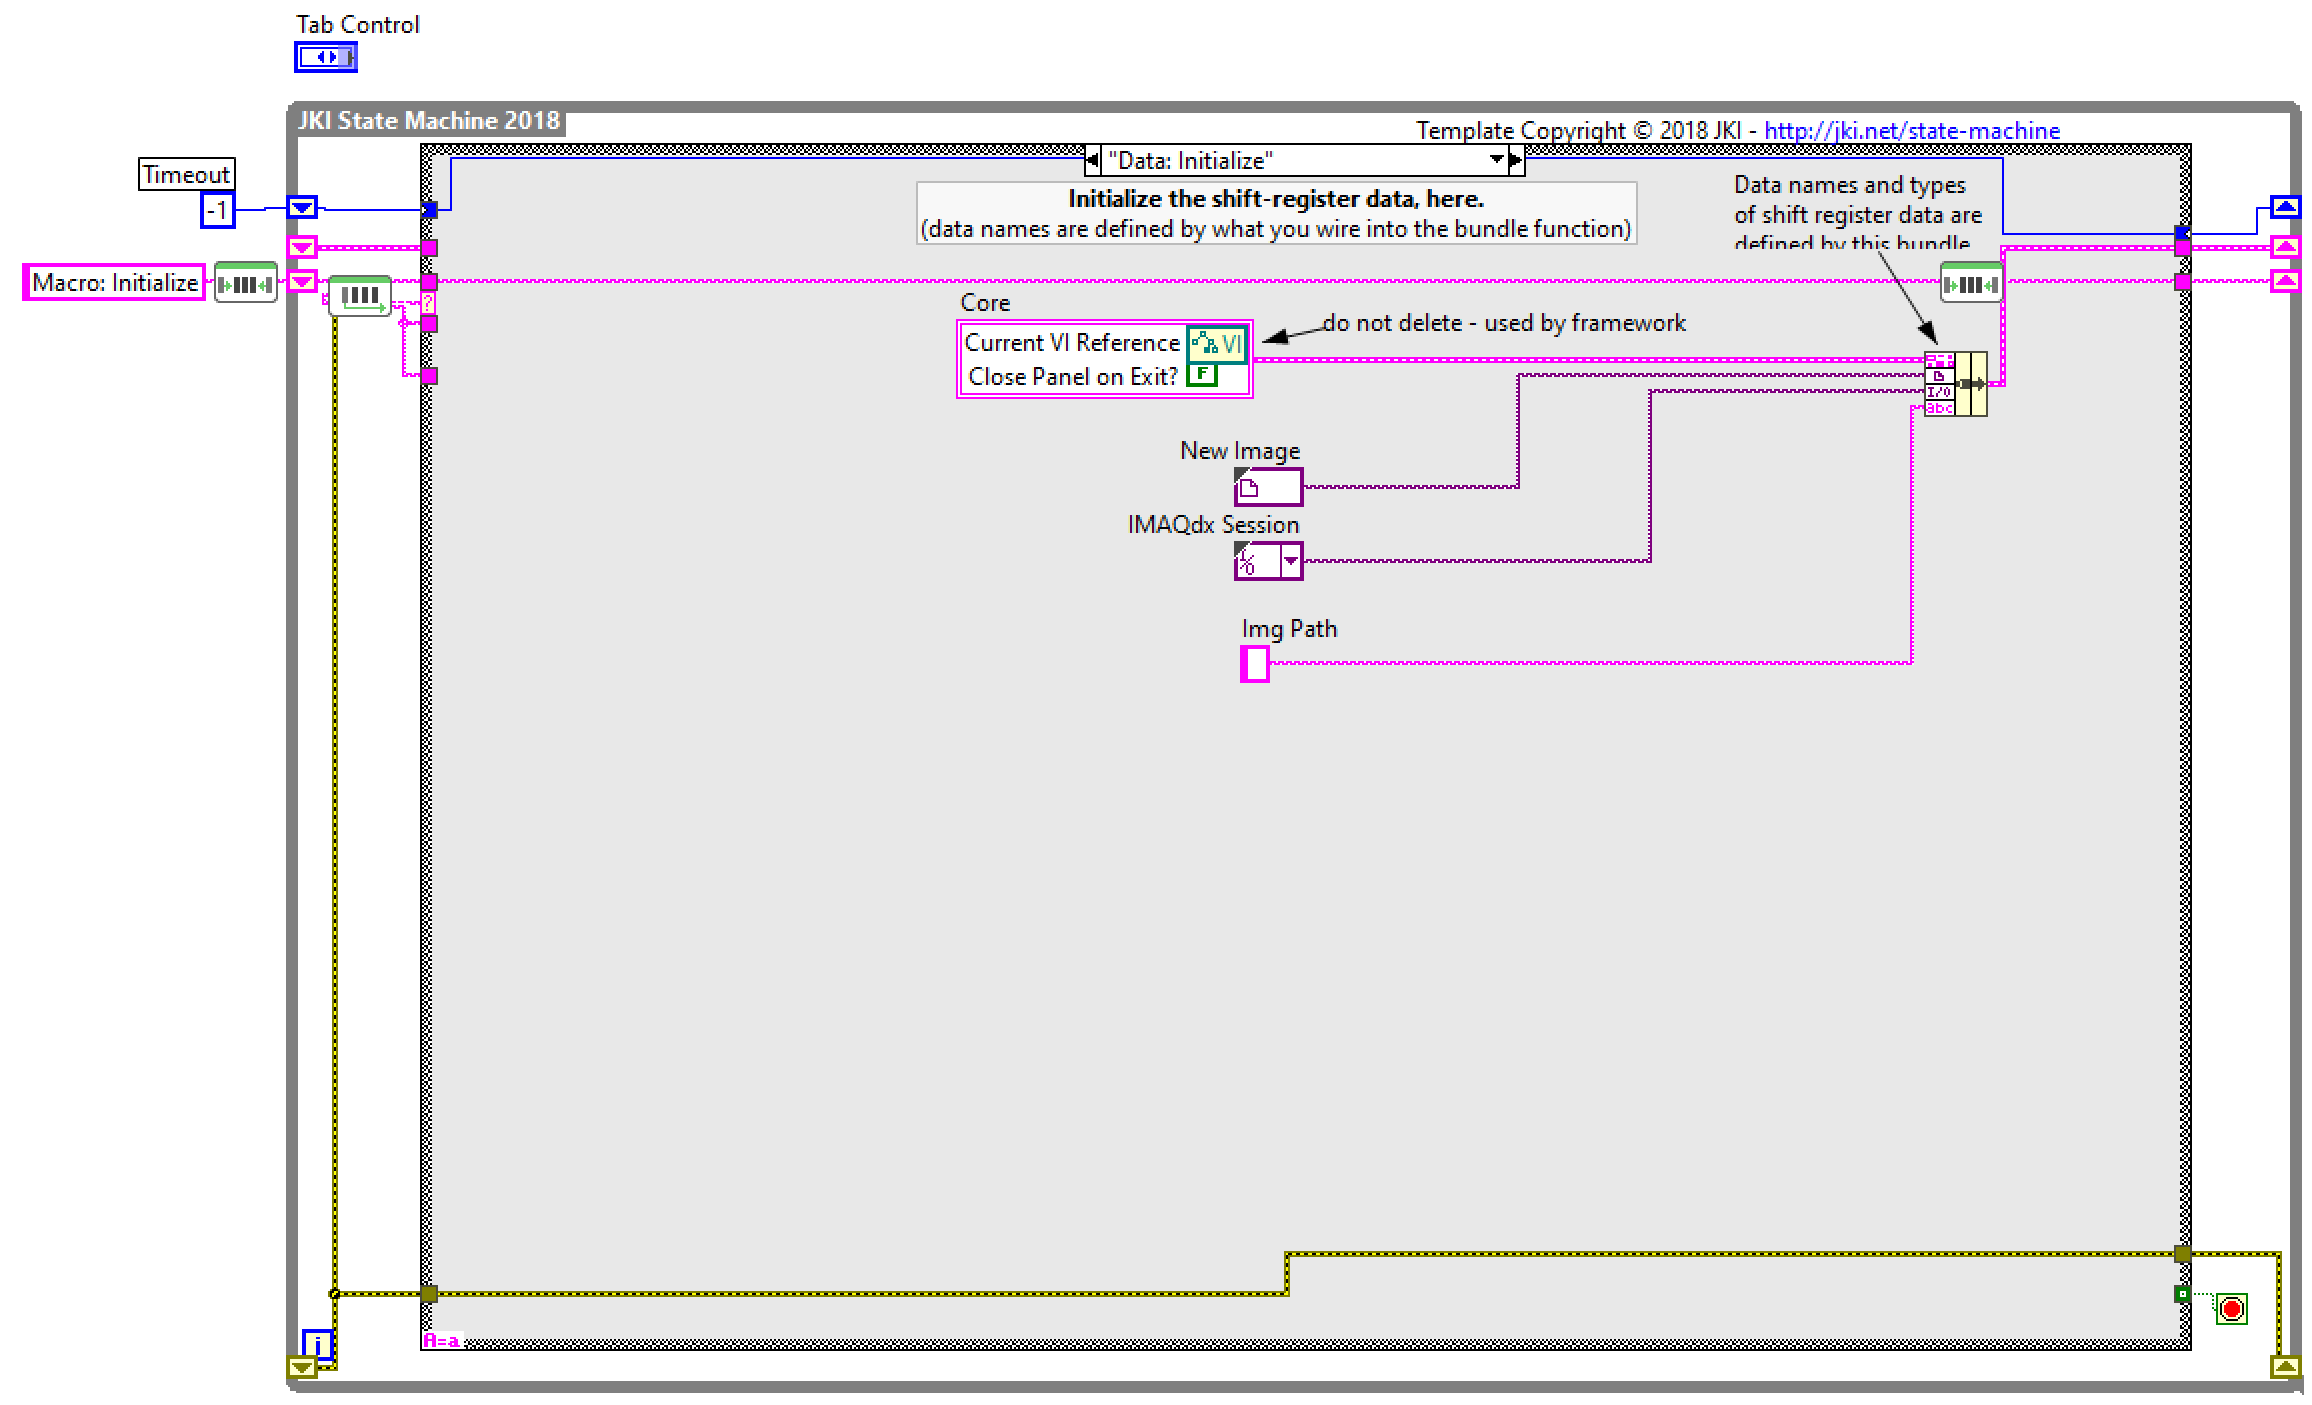
\includegraphics[width=1.0\textwidth]{"src/data-init.png"}
    \caption{Zdjęcie przedstawiające stan "Data: Initialize"}
    \label{fig:foto3}
\end{figure}

Stan "Data: Initialize" odpowiada za inicjalizację żyły zawierającej dane przepływające między stanami. Dzięki wykorzystaniu tej możliwości można przekazywać dowolne dane między kolejnymi stanami oraz modyfikować te dane. 
Dokładne wykorzystanie tej opcji zostanie zaprezentowane w dalszej części dokumentacji. 
Na potrzeby projektu linia danych jest inicjalizowana za pomocą trzech zmiennych:

\begin{itemize}
    \item New Image - przechowuje obraz, jest to zmienna typowa dla biblioteki IMAQ,
    \item IMAQdx Session - kolejna zmienna typowa dla biblioteki IMAQ, przechowuje referencję do otwartek sesji kamery,
    \item Img Path - zmienna typu String przechowująca ściezkę do nowo pobranego zdjęcia.
\end{itemize}

\begin{figure} [H]
    \centering
    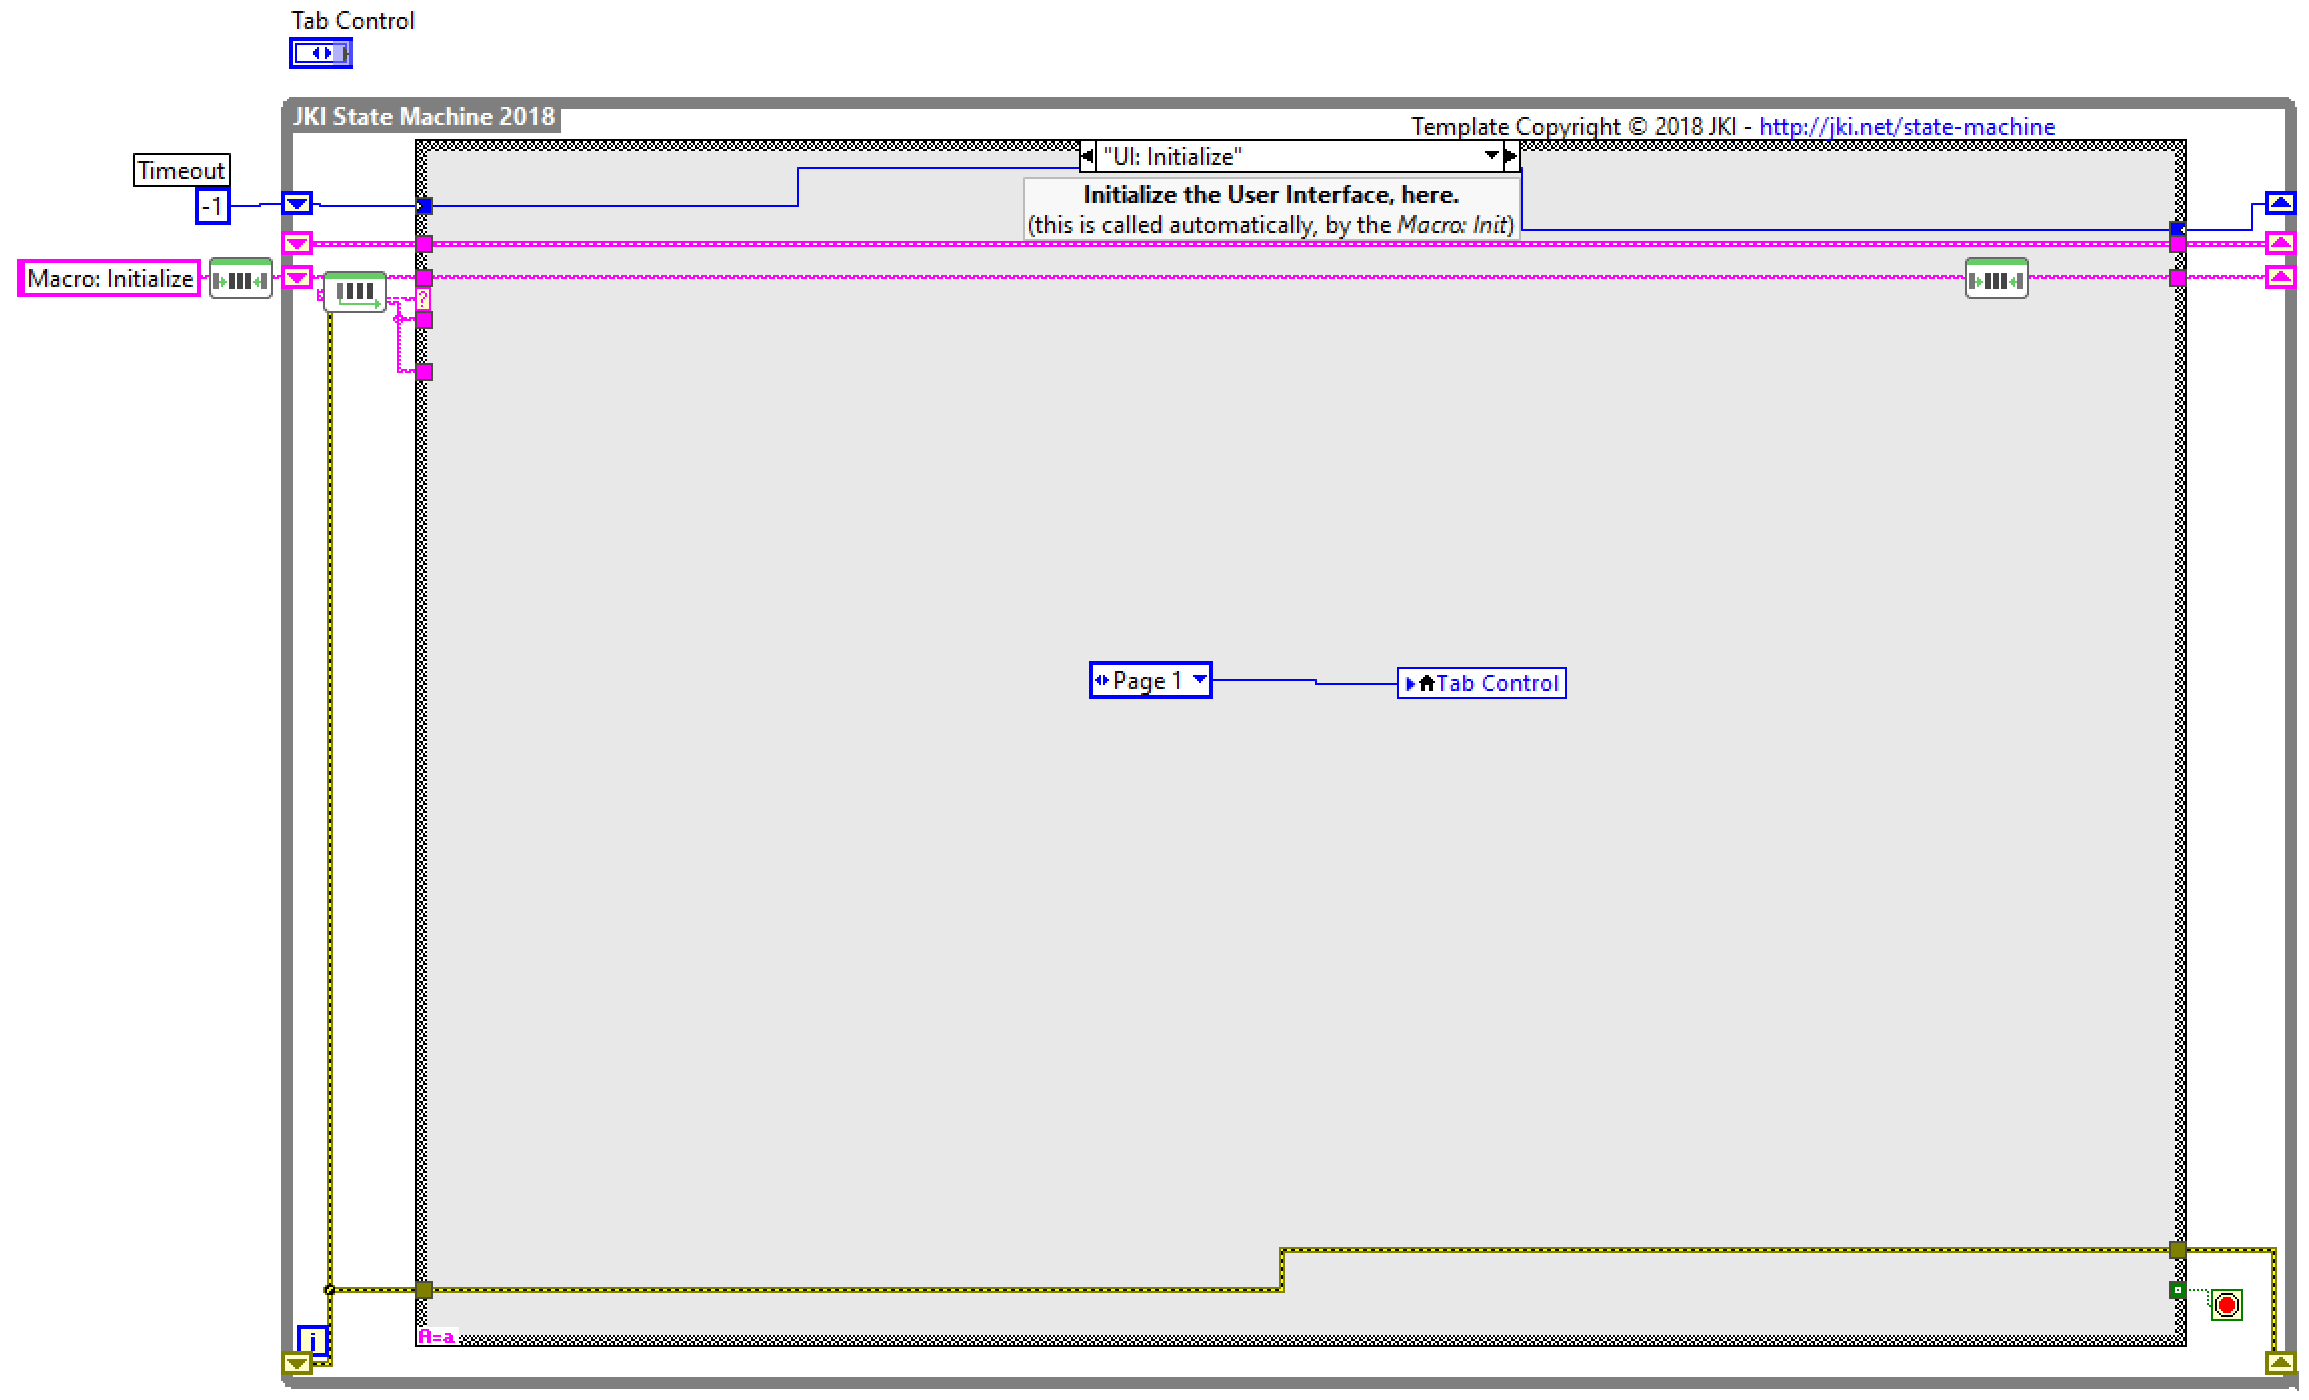
\includegraphics[width=1.0\textwidth]{"src/UI-init.png"}
    \caption{Zdjęcie przedstawiające stan "UI: Initialize"}
    \label{fig:foto4}
\end{figure}

Stan "UI: Initialize" odpowida za wyświetlenie podstawowego widoku aplikacji. W przypadku powyższego projektu odpowiada on za wyświetlenie 
pierwszej zakładki aplikacji przy pomocy struktury Tab dostarczanej przez LabVIEW. 
Element "Page 1" jest standardowym typem wyliczeniowym enum zawierającym deklaracje poszczególnych zakładek. 
Element "Tab Control" odpowiada za wyświetlenie odpowiedniej strony na podstawie wybranej opcji w typie wyliczeniowym.


\subsection{\Large Implementacja procesu logowania w LabView}
Proces logowania jest procesem złożonym z kilku stanów, każdy stan zostanie szczegółowo opisany w poniższej sekcji. 

\subsubsection{\large Stan Face ID: Initialize Grab Image}
Stan "Face ID: Initialize Grab Image" obejmuje procedurę inicjalizacji kamery, niezbędną do późniejszego akwizycji obrazu. W strukturze blokowej tego stanu, centralną rolę pełni struktura "Case", która odpowiada za odpowiednią reakcję aplikacji na wybór kamery. Blok "List Cams" jest opcjonalny, lecz zaleca się jego użycie w przypadku dostępności wielu kamer, umożliwiając użytkownikowi wybór preferowanej. Po dokonaniu wyboru kamery, program przechodzi do kolejnego bloku, który sprawdza dostępność oraz poprawność działania kamery. Z tego bloku wynika binarna flaga, wyznaczająca stan struktury "Case" zgodnie z wynikiem wyboru kamery. Warto zaznaczyć, że blok "Select Camera" zwraca wartość True, jeśli kamera nie została znaleziona lub nie udało się jej poprawnie zainicjalizować; w przypadku powodzenia zwraca False.

W przypadku uzyskania wartości False, odpowiedni stan struktury case zostaje wykonany. Na wejście struktury przekazywane są aktualne stany w kolejce oraz linia Timeout. W centralnej części znajdują się bloki finalizujące konfigurację kamery oraz jej przygotowanie do użycia. Dodatkowo, do linii danych przekazywana jest sesja kamery utworzona przez blok "Configure Grab", oraz pusta referencja do nowego obrazu, który zostanie nadpisany w kolejnym kroku. Ponadto, stan "Face ID: Grab Image" jest dodawany do kolejki jako następny do wykonania.

%  ZDJĘCIE
%
% \begin{figure}[H]
%     \centering
%     includegraphics[width=1.0\textwidth]{}
%     \caption{Zdjęcie przedstawiające stan "Face ID: Initialize Grab Image" jeśli kamera została znaleziona poprawnie}
%     \label{fig:face_id-init_false}
% \end{figure}

Należy zwrócić uwagę na nadpisanie domyślnego Timeout, mające na celu zabezpieczenie aplikacji przed zatrzymaniem w stanie "Idle", czyli bezczynnością.

Jeśli zostanie uzyskana wartość True, a zatem kamera nie została znaleziona, na kolejkę zostaje wysłany stan "Error Handler" oraz wszystkie inne stany zostają usunięte. 
Dodatkowo do linii danych zostaje przesłana pusta referencja do sesji kamery oraz pusta referencja do obrazu. 

Warto zauważyć, że w tym przypadku timeout pozostaje niezmieniony względem jego dymyślnej wartości. 

%  ZDJĘCIE
%
% \begin{figure}[H]
%     \centering
%     includegraphics[width=1.0\textwidth]{}
%     \caption{Zdjęcie przedstawiające stan "Face ID: Initialize Grab Image" jeśli kamera nie została znaleziona poprawnie}
%     \label{fig:face_id-init_false}
% \end{figure}

\subsubsection{\large Stan Face ID: Grab Image}

Stan "Face ID: Grab Image" odpowiada za właściwą akwizycję obrazu oraz jego wyświetlenie na interfejsie użytkownika. 

Pierwszym elementem widoczym na schemacie blokowym jest blok "Unbundle by Name", który odpowiada za wyodrędnienie danych przesyłanych poprzez linię danych jako klaster. Drugim elementem jest przycisk, mający na celu rozpoczęcie akwizycji obrazu. W centralnym punkcie schematu znajduje się blok "Take Image Case Struct". Jest to plik SubVi, który przechowuje logikę pobierania obrazu. Na wejścia tego bloku należy poprowadzić:
\begin{itemize}
    \item IMAQdx Session - aktualną sesję kamery,
    \item New Image - Referencję do obrazu,
    \item Przycisk odpowiedzialny za rozpoczęcie procesu logowania,
    \item Error In - Błąd.
\end{itemize}

Na wyjściach bloku znajdują się:
\begin{itemize}
    \item IMAQdx Session - Aktualną sesję kamery,
    \item New Image - Referencję do pobranego obrazu,
    \item Kolejne stany do kolejki,
    \item Error Out - Błąd wyjściowy.
\end{itemize}

Kolejnym istotnym elementem jest blok Image Display, odpowiada on za wyświetlenie pobranego obrazu na interfejsie użytkownika.

Ostatnim elementem znajdującym się na schemacie jest blok "Bundle By Name", którego działanie jest odwrotne do działania bloku "Unbundle By Name", zatem tworzy on klaster danych poprzez połączenie kilku danych wejściowych.

% ZDJĘCIE
%
% \begin{figure}[H]
%     \centering
%     includegraphics[width=1.0\textwidth]{}
%     \caption{Zdjęcie przedstawiające stan "Face ID: Grab Image"}
%     \label{fig:face_id-init_false}
% \end{figure}

\subsection*{Take Image Case Struct - SubVi}

Jak wspomniano wcześniej, powyższy SubVi odpowiada za logikę pobrania zdjęcia. Ze względu na dbałość o czyistość i przejrzystość kodu w przypadku dużej ilości bloków, należy starać się wyodrębnić część bloków do SubVi właśnie. Naturalnie wejścia oraz wyjścia są takie same jak opisane wyżej, dlatego nie będą ponownie wyszczególniane. 

Rdzeniem tego SubVi jest struktura Case, która na podstawie stanu przycisku odpowiednio wykonuje stan True lub False. 
Jeśli stan przycisku jest równy False, obraz jest pobierany przez blok "Get Image2", a następnie przekazywany na wyjście wraz z trwającą sesją kamery. Natomiast do kolejki zostaje przekazany stan "Face ID: Grab Image", co oznacza zapętlenie maszyny stanów w tym stanie dopóki nie nastąpi naciśnięcie przycisku "Exit" kończącego działanie całej aplikacji lub nie zostanie naciśnięty przycisk logowania. 

W przypadku naciśnięcia przycisku logowania, zostaje wykonany stan True. Proces pobierania obrazu oraz przekazywania jego referencji na wyjście jest niezmieniony. Różnica pojawia się natomiast w sposobie przekazywania kolejnego stanu do kolejki. Poczynając od środka, można zauważyć blok "Elapsed Time", jest on odpowiedzialny za licznik, który określa jak długo ma trwać akwizycja danych. Jeśli licznik jest w trakcie odliczania, na jego wyjściu pojawia się flaga "False" i trafia na blok "Select", który jest odpowiedzialny za wybór odpowiedniej wartości na podstawie warunku. Można porównać ten blok do prostej instrukcji warunkowej if. Zatem jeśli licznik jest w trakcie działania, do kolejki jest przekazywany stan "Face ID: Grab Image" oraz grupa stanów "Event Structure". To oznacza, że ponownie tak długo jak trwa timer, aplikacja będzie zapętlona na stanie "Face ID: Grab Image". W momencie, gdy licznik zwróci wartość True - odliczy zadany czas, do kolejki zostaje przekazany stan "Face ID: Stop Grab Image". 

% ZDJĘCIE
%
% \begin{figure}[H]
%     \centering
%     includegraphics[width=1.0\textwidth]{}
%     \caption{Zdjęcie przedstawiające SubVI Take Image Case Struct}
%     \label{fig:face_id-init_false}
% \end{figure}

\subsubsection{\large Stan Face ID: Stop Grab Image}

Następny stan odpowiada za zatrzymanie akwizycji obrazu oraz usunięcie nieużywanych referencji w celu zwolnienia zasobów komputera.

Pierwszą wykonywaną funkcją jest wyodrębnienie danych z klastra pochodzącego z linii danych. Następnie, trwająca sesja kamery zostaje przekazana jako parametr wejściowy dla bloku "Stop Acquisition". Sesja kamery jest następnie przekazywana do bloków "Unconfigure Camera" oraz "Close Camera". Ta sekwencja jest konieczna do poprawnego zamknięcia kamery. Jeśli nie wszystkie kroki zostaną wykonane, istnieje ryzyko, że kamera będzie niewidoczna lub niedostępna dla innych aplikacji z powodu nieusuniętej referencji utworzonej przez aplikację LabVIEW.

Referencja do obrazu zostaje przekazana do bloku "Save Image". Zapis obrazu jest konieczny ze względu na późniejszą analizę zarejestrowanego obrazu oraz weryfikację tożsamości. Następnie referencja jest usuwana przy użyciu bloku "Imaq Dispose".

Warto zauważyć sposób przekazania ścieżki do zapisu zarejestrowanego obrazu. W celu większej elastyczności programu zastosowane zostały ścieżki względne. Budowa ścieżki względnej rozpoczyna się od użycia bloku "Current VI's Path", zwracającego ścieżkę bezwzględną do aktualnej lokalizacji VI. Następnie odpowiednio dodawana jest stała typu "Path Constant", w taki sposób, aby otrzymać pożądaną lokalizację. Następnie używany jest blok "Build Path", który konkatenuje obie składowe, tworząc poprawną ścieżkę.

Do linii danych przekazywana jest pusta referencja do sesji kamery, przygotowując system na ewentualne ponowne użycie kamery. Do kolejki przekazywany jest kolejny stan "Face ID: Image Processing".

Ponieważ niebezpieczeństwo zablokowania aplikacji podczas używania kamery przestaje obowiązywać po jej zamknięciu, zostaje włączony domyślny timeout.

Dodatkowo, następuje przejście z zakładki "Page 1" do zakładki "Page 2" za pomocą bloku "Tab Control", do którego na wejście przekazywana jest odpowiednia wartość typu wyliczeniowego zawierającego istniejące zakładki.

% ZDJĘCIE
%
% \begin{figure}[H]
%     \centering
%     includegraphics[width=1.0\textwidth]{}
%     \caption{Zdjęcie przedstawiające stan Face ID: Stop Grab Image}
%     \label{fig:face_id-init_false}
% \end{figure}

\subsubsection{\large Stan Face ID: Image Processing}

Ostatni stan związany z procesem logowania to "Face ID: Image Processing". Proces identyfikacji użytkownika rozpoczyna się od bloku "Open Python Session", który przygotowuje środowisko uruchomieniowe LabVIEW do użycia języka Python. Na wejście bloku należy podać błąd, wersję języka Python oraz ścieżkę do pliku wykonywalnego .exe uruchamiającego kompilator. Na wyjściu pojawi się sygnał zawierający aktualną sesję Python oraz ewentualny błąd.

Następnie następuje właściwe wywołanie funkcji realizującej porównanie. Na wejście bloku "Python Node" należy podłączyć otwartą wcześniej sesję oraz ścieżkę do miejsca, w którym znajduje się skrypt. Ścieżka została zaimplementowana za pomocą bloku "Path Builder". Opcjonalnie blok "Python Node" można rozciągnąć, aby pokazały się puste pola, które obrazują argumenty wejściowe funkcji oraz typ wartości zwracanej. W aktualnej wersji aplikacji do wymienionego bloku została podłączona stała typu Boolean, co wskazuje na typ wartości zwracanej. Argumenty wejściowe nie są wymagane w obecnej wersji aplikacji.

Po zakończeniu działania sesja Python zostaje zamknięta, a wartość zwrócona z funkcji \newline \texttt{find\_face\_encodings} wywołuje odpowiedni stan struktury case. Jeśli proces logowania został zakończony sukcesem, wykonuje się case "True" - wyświetlana jest informacja na ekranie użytkownika o statusie logowania, a do kolejki zostaje przekazany kolejny stan, którym jest "Face ID: Control Panel". Następuje również przełączenie na trzecią zakładkę za pomocą bloku "Tab Control".

W przypadku, gdy logowanie nie zakończyło się sukcesem, wyświetlana jest informacja o statusie logowania, a do kolejki zostaje przekazany stan "Face ID: Initialize Grab Image", co powoduje, że aplikacja wraca do stanu początkowego. Zakładka zostaje przełączona na ekran początkowy.
 
%
% \begin{figure}[H]
%     \centering
%     includegraphics[width=1.0\textwidth]{}
%     \caption{Zdjęcie przedstawiające stan Face ID: Image Processing}
%     \label{fig:face_id-init_false}
% \end{figure}

\subsection{\Large Implementacja identyfikacji użytkownika}

Funkcja \texttt{find\_face\_encodings} realizuje proces porównania twarzy w celu identyfikacji użytkownika. Działanie funkcji można podzielić na kilka kluczowych kroków.

Na początku, funkcja definiuje ścieżkę do folderu z zarejestrowanymi użytkownikami oraz wczytuje tymczasowy obraz logowania za pomocą biblioteki \texttt{cv2}. 

Następnie, za pomocą funkcji \texttt{face\_recognition.face\_encodings}, funkcja przetwarza wczytany obraz w celu ekstrakcji cech twarzy. Jeżeli w obrazie nie zostanie wykryta twarz, funkcja zwraca wartość \texttt{False} i kończy działanie, informując o braku wykrycia twarzy.

Funkcja iteruje przez wszystkie pliki graficzne znajdujące się w folderze z zarejestrowanymi użytkownikami. Dla każdego obrazu próbuje wyodrębnić cechy twarzy. Jeżeli w obrazie nie zostanie wykryta twarz, funkcja kontynuuje przetwarzanie kolejnych plików, informując o niepowodzeniu detekcji dla danego pliku.

Dla każdej zarejestrowanej twarzy, funkcja porównuje jej kodowanie z kodowaniem twarzy z obrazu logowania za pomocą funkcji \texttt{face\_recognition.compare\_faces}. Jeżeli zostanie znalezione dopasowanie, funkcja oblicza odległość pomiędzy kodowaniami twarzy przy użyciu funkcji \newline \texttt{face\_recognition.face\_distance} oraz przekształca tę odległość na poziom dokładności (accuracy).

Jeżeli funkcja znajdzie dopasowanie, informuje o sukcesie porównania, wyświetlając nazwę dopasowanego pliku oraz poziom dokładności. Funkcja zwraca wartość \texttt{True}, sygnalizując pomyślne logowanie użytkownika. 

Jeżeli żadne z kodowań twarzy z zarejestrowanych obrazów nie będzie zgodne z kodowaniem twarzy z obrazu logowania, funkcja zwraca wartość \texttt{False}, informując o niepowodzeniu procesu logowania.

Funkcja \texttt{find\_face\_encodings} jest kluczowym elementem systemu rozpoznawania twarzy, odpowiadającym za porównanie twarzy użytkownika z bazą zarejestrowanych obrazów. Wykorzystując biblioteki \texttt{cv2} oraz \texttt{face\_recognition}, funkcja ta skutecznie identyfikuje użytkownika, zapewniając odpowiedni poziom dokładności i niezawodności.

\subsection{\Large Implementacja procesu dodawania użytkownika}

\subsubsection{\large Stan Add User: Input Image Init}

%% Opis procesu dodawania użytkownika zrealizować tak samo jak proces logowania,
%% Być może nieco mniej szczegółowo

\subsection{\Large Implementacja połączenia aplikacji z bazą danych}

%% Opis podobnie jak wcześniej jednak szczegółowo ze względu na nieco większą złożoność

\section{\LARGE Napotkane problemy}
\subsection{\Large Implementacja zakładek}

\subsection{\Large Wywoływanie skryptów Python z poziomu LabVIEW}

\subsection{\Large Wykonanie działającego połączenia aplikacji z bazą danych SQL}

\section{\LARGE Podsumowanie}

\end{document}
